\section{Temporal Analyses}
\label{sec:3_4_results}

In this section I show different analysis to discover and characterize how the FFCS are used. In the first part of the section, I analyse the temporal systems characterization to understand if FFCS are actually used and when.

I consider a period from December 10th 2016 to January 31st 2017, the first reliable collected data chunk. The system observed 125,000 snapshots, about 104,000 bookings for car2go and 93,000 for Enjoy. In Turin, the fleet of car2go was composed by 394 cars, and the fleet of Enjoy was composed by 172 cars.

In order to make clear the rest of the book, it necessary to univocally define the basilar entities related to the car status in the data lake defined in the chapter \ref{chap:2_dataset}, section \ref{sec:2_4_data_normalization}.

\begin{definition}{the \textbf{Parking}}
	\label{def:parking} is the time period in which the car is present in, at least, two consecutive snapshot. Therefore that car it is available for an user reservation
\end{definition}
\begin{definition}{the \textbf{Booking}}
	\label{def:booking} is the time period in which the car is NOT present in, at least, two consecutive snapshot. There fore an user booked that vehicle or the provider temporary removed it for maintenance.
\end{definition}


\subsection{System Utilization}

\begin{figure}
\centering
 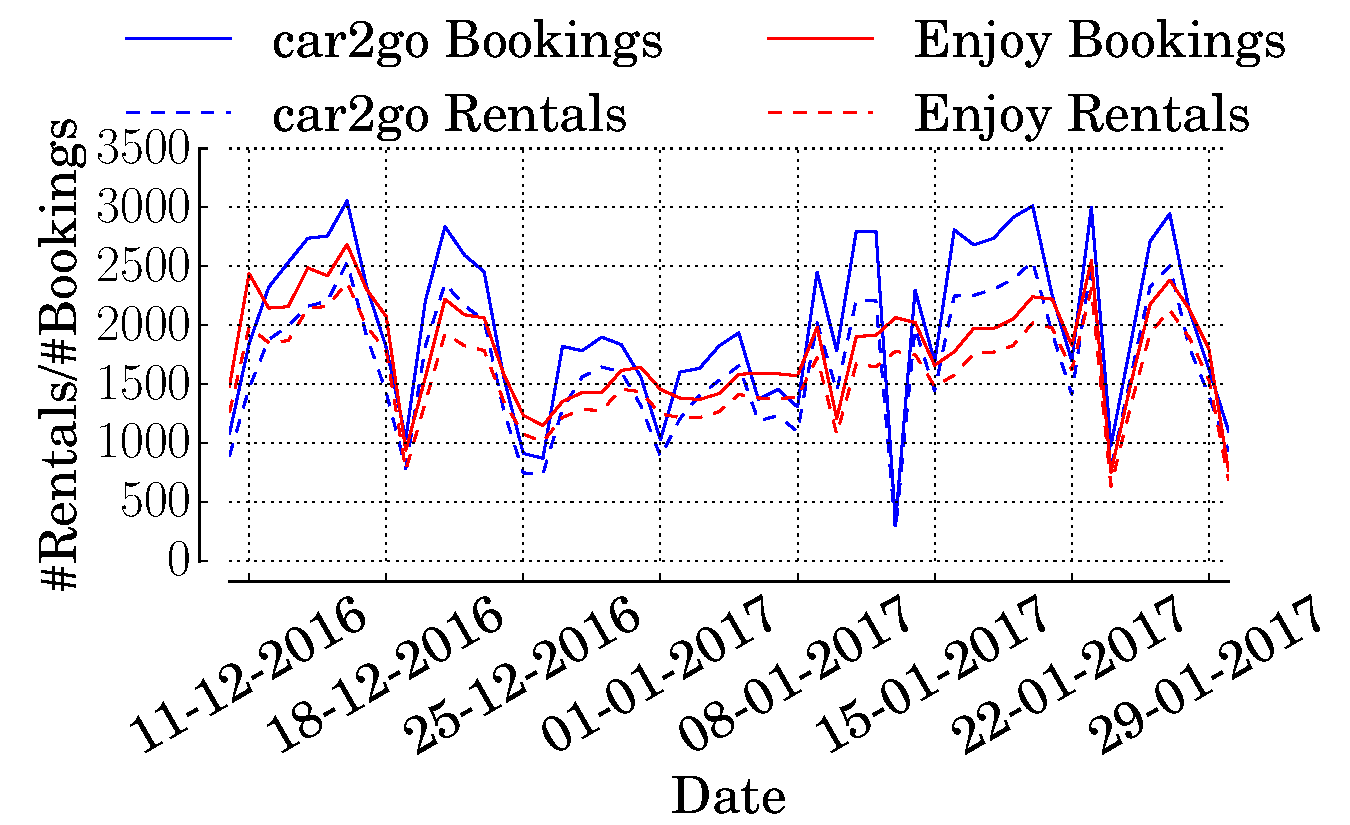
\includegraphics[ width=0.65\columnwidth]{figures/bookings.pdf}
 \caption{Total number of bookings and of rentals per day for car2go and for Enjoy \label{fig:3_4_bookings}}
\end{figure}
The providers, in this case study, allows the users to \textit{reserve} a car before the ride. More in details, the provider makes the reserved car unavailable for the other users without billing the customer who reserved the car. When the reservation time (that changes for each provider), the billing mechanism starts even if the engine it is still off. The customer can cancel the reservation without any expense if it happens before the reservation time. With this mechanism, the providers would let the possibility to the users to reach the cars by foot.

Given that, it is now possible to the define:
\begin{definition}{\textbf{Reservation}}
	\label{def:reservation} A reservation it is a booking where the initial and final destination matches and the duration is lower than the provider's reservation time.
\end{definition}

\begin{definition}{\textbf{Rental}}
	\label{def:rental} A rental it is a booking where the initial and final destination are different.
\end{definition}


Starting from December 10th, figure~\ref{fig:3_4_bookings} plots the total number of bookings and the total number of rentals recorded on each day, for car2go (blue curves), and for Enjoy (red curves). Obviously, being the latter a subset of the first, its number is always smaller. However, during some days, the discrepancy is well visible; that means that the operation of booking cancellation is not so rare.

Interestingly, firstly, both car2go and Enjoy follow a similar behaviour with the number of bookings and rentals decreasing in the Christmas period and increasing again after the Epiphany. 

Secondly, despite car2go fleet has more than twice as much cars than Enjoy (394 vs. 172), the number of car2go bookings does not show such a higher value with respect to Enjoy. With Enjoy having more bookings in some snapshots e.g., December 10th and 11th. Moreover, in some points (ecember 19th, January 24th) it is possible to detect huge drop due to the crawler failures. 

Moreover, some drops in bookings' values are noticeable. Those sudden changes can be addressed to some failures, in the crawlers (e.g., when all curves suddenly drop) or in the operators' web services(e.g., when only one system suffers a sudden drop).



\begin{figure}
\centering
 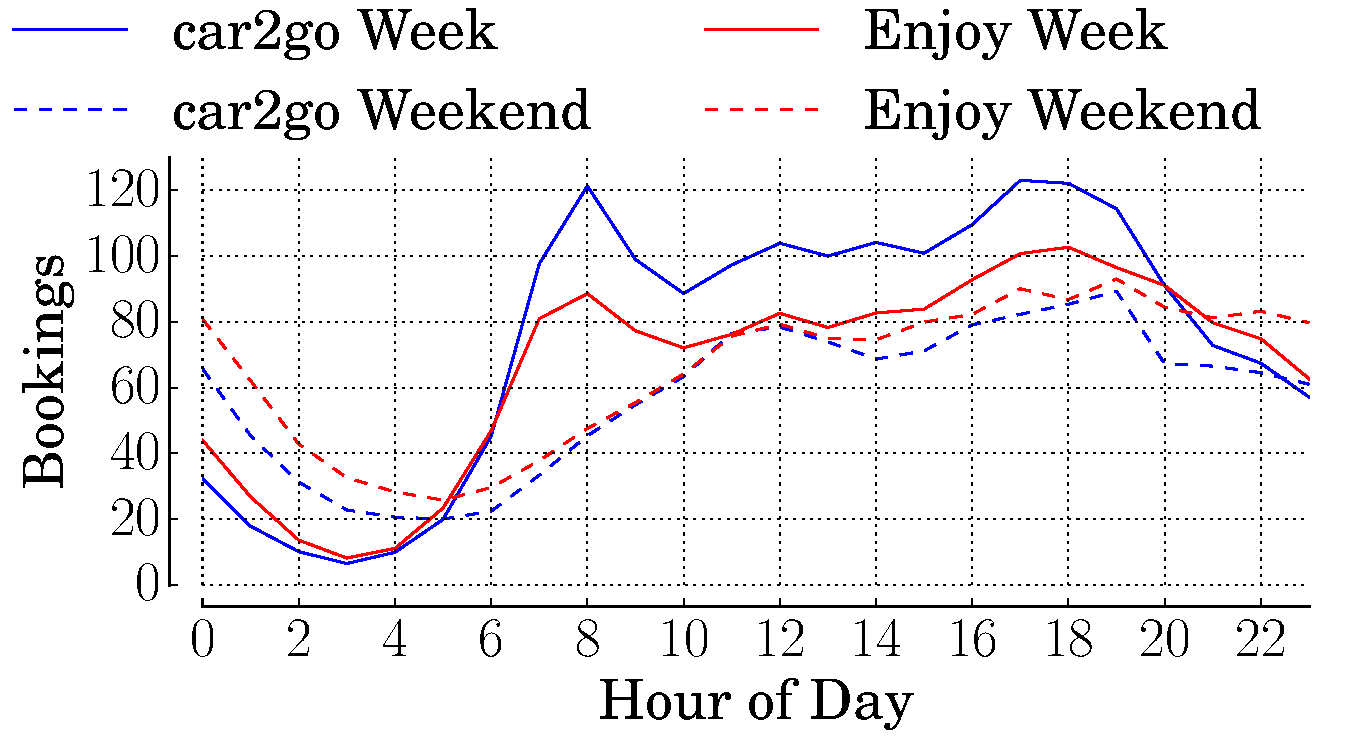
\includegraphics[ width=0.65\columnwidth]{figures/bookings_day.pdf}
 \caption{Mean number of bookings in weekdays and weekends for car2go and Enjoy\label{fig:3_4_bookingsweek}}
\end{figure}

Looking at the data with a finer granularity, it is noticeable that the car sharing adoption changes during the day. To better characterize this, I separate weekdays and weekends. The figure~\ref{fig:3_4_bookingsweek} points out the trend over the day. The curves report the average number of bookings over the entire period  in each hour of the day.

Firstly, it is possible to see that weekdays and weekends have a quite different trend. During the weekend FFCS systems are more used at night with respect than weekdays, with on average at midnight of 80 and 60 bookings per hour for Enjoy and car2go. Instead, the figure shows how during the weekdays both car2go and Enjoy have their peak of usage at 8~am and between 5~pm and 7~pm. This trend can be easily explained as, during that time slots, FFCS customers use cars to go and return from work. 
As previously indicated, despite car2go has twice the number of cars than Enjoy, the system utilization of the latter is higher, with peak utilization topping to 60\%, versus 30\% of car2go. 

Even in absolute number of rentals, Enjoy shows an higher number of bookings after 8~pm during the weekdays, and always during the weekends. This can be explained by the car models adopted by the two companies. While car2go uses the compact-two seats \textit{Smart}, Enjoy fleet is composed of \textit{Fiat 500}, which are 4 seats cars. Rentals prices are instead comparable (0.24\euro/min Enjoy vs 0.25\euro/min car2go). Data suggests that Enjoy looks more appealing during the times when people prefer to share the ride, and during weekends when families and groups move. 